% Options for packages loaded elsewhere
\PassOptionsToPackage{unicode}{hyperref}
\PassOptionsToPackage{hyphens}{url}
%
\documentclass[
]{article}
\usepackage{amsmath,amssymb}
\usepackage{iftex}
\ifPDFTeX
  \usepackage[T1]{fontenc}
  \usepackage[utf8]{inputenc}
  \usepackage{textcomp} % provide euro and other symbols
\else % if luatex or xetex
  \usepackage{unicode-math} % this also loads fontspec
  \defaultfontfeatures{Scale=MatchLowercase}
  \defaultfontfeatures[\rmfamily]{Ligatures=TeX,Scale=1}
\fi
\usepackage{lmodern}
\ifPDFTeX\else
  % xetex/luatex font selection
\fi
% Use upquote if available, for straight quotes in verbatim environments
\IfFileExists{upquote.sty}{\usepackage{upquote}}{}
\IfFileExists{microtype.sty}{% use microtype if available
  \usepackage[]{microtype}
  \UseMicrotypeSet[protrusion]{basicmath} % disable protrusion for tt fonts
}{}
\makeatletter
\@ifundefined{KOMAClassName}{% if non-KOMA class
  \IfFileExists{parskip.sty}{%
    \usepackage{parskip}
  }{% else
    \setlength{\parindent}{0pt}
    \setlength{\parskip}{6pt plus 2pt minus 1pt}}
}{% if KOMA class
  \KOMAoptions{parskip=half}}
\makeatother
\usepackage{xcolor}
\usepackage{graphicx}
\makeatletter
\def\maxwidth{\ifdim\Gin@nat@width>\linewidth\linewidth\else\Gin@nat@width\fi}
\def\maxheight{\ifdim\Gin@nat@height>\textheight\textheight\else\Gin@nat@height\fi}
\makeatother
% Scale images if necessary, so that they will not overflow the page
% margins by default, and it is still possible to overwrite the defaults
% using explicit options in \includegraphics[width, height, ...]{}
\setkeys{Gin}{width=\maxwidth,height=\maxheight,keepaspectratio}
% Set default figure placement to htbp
\makeatletter
\def\fps@figure{htbp}
\makeatother
\setlength{\emergencystretch}{3em} % prevent overfull lines
\providecommand{\tightlist}{%
  \setlength{\itemsep}{0pt}\setlength{\parskip}{0pt}}
\setcounter{secnumdepth}{-\maxdimen} % remove section numbering
\ifLuaTeX
  \usepackage{selnolig}  % disable illegal ligatures
\fi
\usepackage{bookmark}
\IfFileExists{xurl.sty}{\usepackage{xurl}}{} % add URL line breaks if available
\urlstyle{same}
\hypersetup{
  pdftitle={阅读1},
  hidelinks,
  pdfcreator={LaTeX via pandoc}}

\title{阅读1}
\author{}
\date{}

\begin{document}
\maketitle

\section{DDM}\label{ddm}

\begin{quote}
quote from Yang Song\\
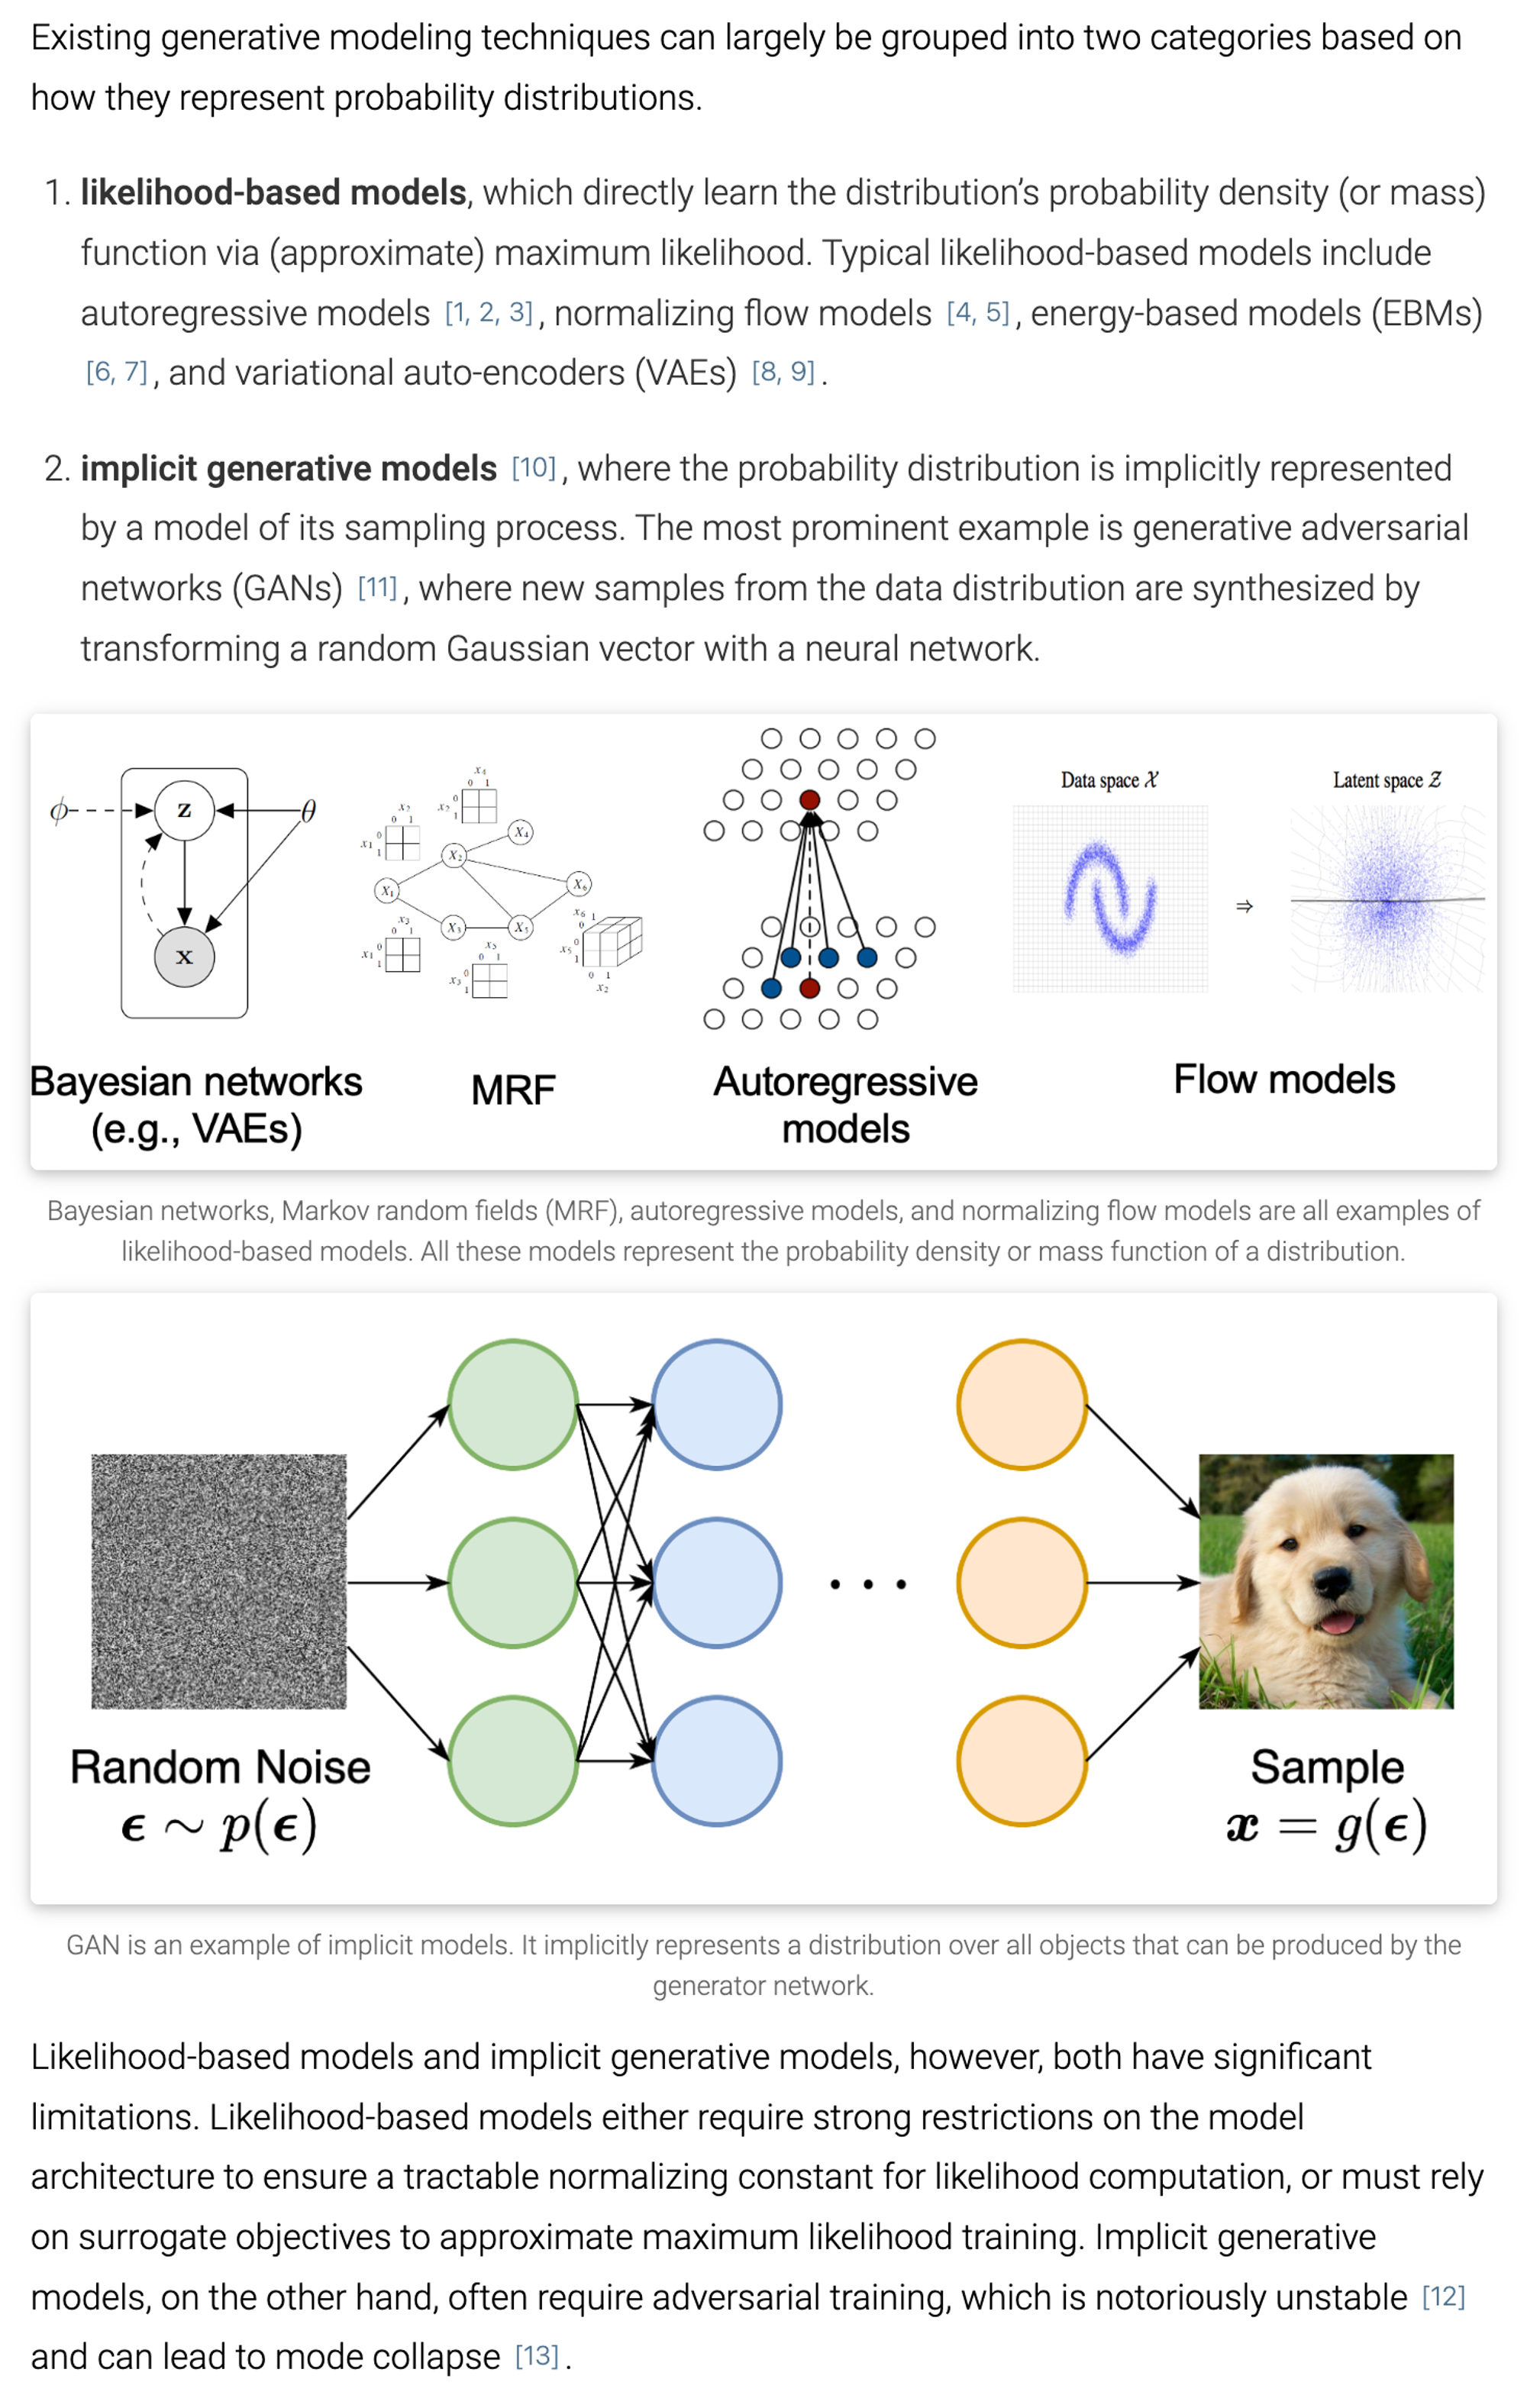
\includegraphics{E:/Learning/MyObsidian/MyObsidian/Pasted image 20240116102851.png}
\end{quote}

\subsection{BG}\label{bg}

\begin{itemize}
\tightlist
\item
  generated by latent variable {}
\item
  generally learn low-dim latent representations
\end{itemize}

\subsubsection{ELBO}\label{elbo}

\begin{enumerate}
\item
  {}: model the latent variable and the data, likelihood-based: maximize
  the likelihood {}.
\item
  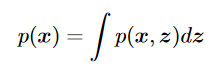
\includegraphics{E:/Learning/MyObsidian/MyObsidian/Pasted image 20231129170724.png}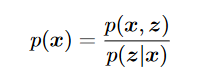
\includegraphics{E:/Learning/MyObsidian/MyObsidian/Pasted image 20231129170731.png}
\item
  推导evidence lower bound:(VLB ELB)

  \begin{enumerate}
  \tightlist
  \item
    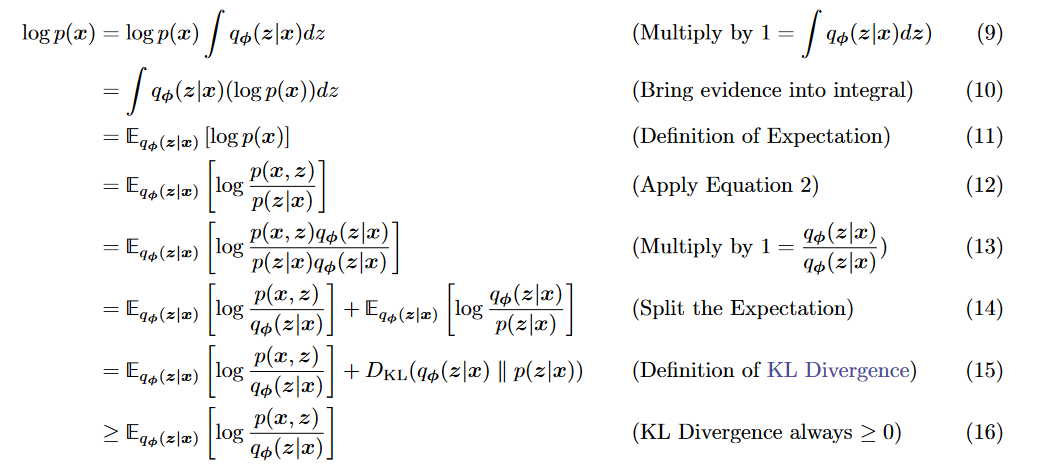
\includegraphics{E:/Learning/MyObsidian/MyObsidian/Pasted image 20231129171149.png}KL大于0,
    {}: the approximate posterior.p(x):likelihood of observed or
    generated data
    当KL趋近于0意味着logp(x)接近于ELBO式。如果减小KL距离,则q接近真实后验分布。但因为我们不知道真实后验,所以KL很难计算。而左侧p(x)与参数{}无关,所以optimize
    ELBO就等于使得估计的后验
    接近真实的后验。并且因为KL趋近于0,可以用ELBO估计p(x)
  \end{enumerate}
\end{enumerate}

\subsubsection{VAE}\label{vae}

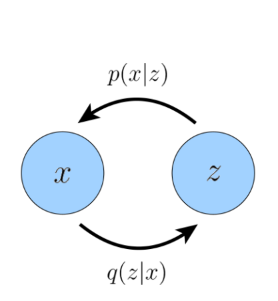
\includegraphics{E:/Learning/MyObsidian/MyObsidian/Pasted image 20240223102231.png}

\begin{enumerate}
\tightlist
\item
  maximize ELBO

  \begin{enumerate}
  \tightlist
  \item
    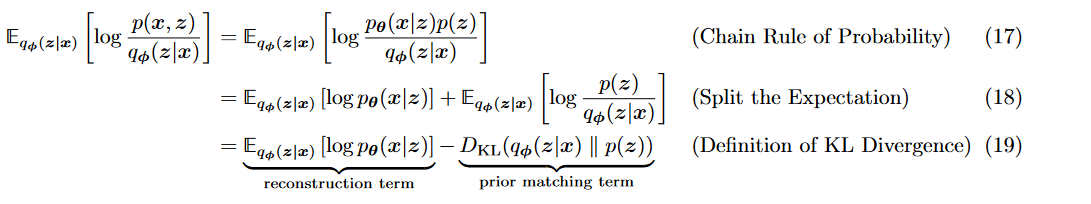
\includegraphics{E:/Learning/MyObsidian/MyObsidian/Pasted image 20231129172419.png}

    \begin{enumerate}
    \tightlist
    \item
      encoder learn {}, decoder learn {}
    \end{enumerate}
  \end{enumerate}

  \begin{itemize}
  \tightlist
  \item
    式子

    \begin{itemize}
    \tightlist
    \item
      reconstruction likelihood of decoder:确保decoder对latent有效建模
    \item
      学习到的 z 分布(variational distribution)
      (q(z\textbar x))和先验相似程度。确保encoder有效建模而不是一个Dirac函数
    \end{itemize}
  \end{itemize}
\item
  encoder: 学习一个multi gaussion, 假设prior是standard gaussion:

  \begin{enumerate}
  \tightlist
  \item
    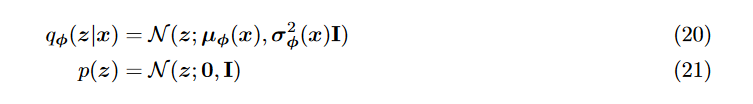
\includegraphics{E:/Learning/MyObsidian/MyObsidian/Pasted image 20231129173604.png}
  \item
    reconstruction term 可以用monte varlo估计,latents {} are sampled
    from {} .单纯sample是不可导的-\textgreater{} reparamterization trick
  \item
    reparamterization trick: 将r.v.重写做noise
    variable函数,从而化为从一个standard gaussioan
    中sample,能够对参数做gradient descent.(注意 {} element-wise
    product)\\
    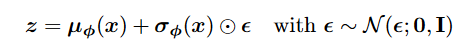
\includegraphics{E:/Learning/MyObsidian/MyObsidian/Pasted image 20231129174306.png}
  \item
    VAE中 z dim 小于x-\textgreater 学到compact latent vector,
    可修改latent vector控制生成
  \end{enumerate}
\end{enumerate}

\subsubsection{HVAE}\label{hvae}

将前向反向都看作为马尔科夫链: decoding each latent {} only conditions
on previous latent {}, 低级依赖高级

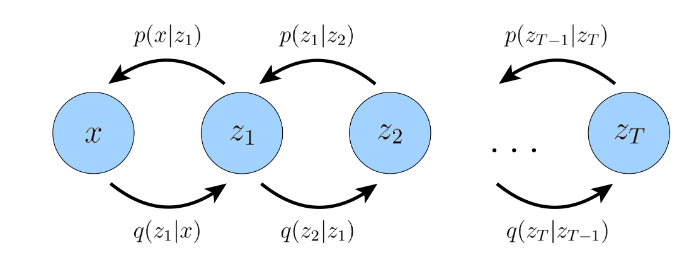
\includegraphics{E:/Learning/MyObsidian/MyObsidian/Pasted image 20231129205321.png}\\
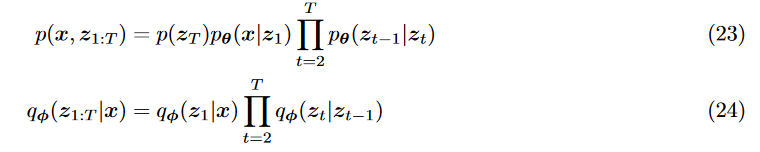
\includegraphics{E:/Learning/MyObsidian/MyObsidian/Pasted image 20231129205331.png}\\
Lower-bound:\\
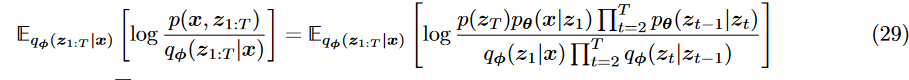
\includegraphics{E:/Learning/MyObsidian/MyObsidian/Pasted image 20231129205414.png}

\subsection{Variational Diffusion
Models}\label{variational-diffusion-models}

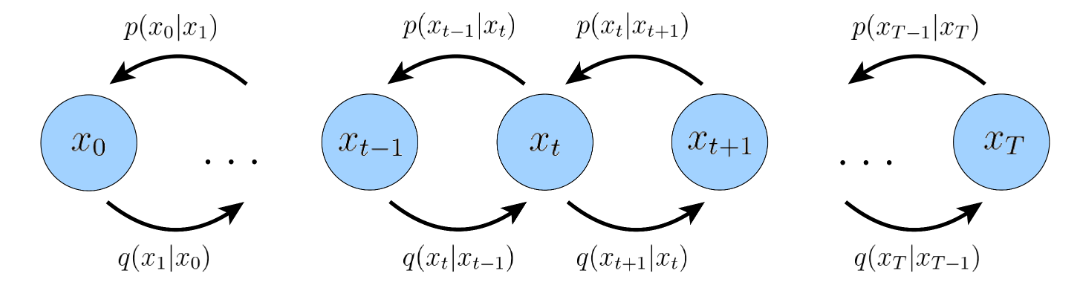
\includegraphics{E:/Learning/MyObsidian/MyObsidian/Pasted image 20231129205937.png}

\begin{enumerate}
\tightlist
\item
  与HVAE不同

  \begin{enumerate}
  \tightlist
  \item
    latent dim = data dim (所以latent 和data 都写作{} )
  \item
    at t, the latent encoder is defined as a linear Gaussian model
  \item
    The Gaussian parameter of latent encoder vary -\textgreater{} at
    final T, standard Gaussian
  \end{enumerate}
\item
  the distribution of each latent variable in the encoder is a Gaussian
  centered around its previous hierarchical latent.

  \begin{enumerate}
  \tightlist
  \item
    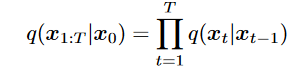
\includegraphics{E:/Learning/MyObsidian/MyObsidian/Pasted image 20231129210136.png}
  \item
    linear Gaussian parameters: hyperparameters or learned
  \item
    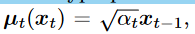
\includegraphics{E:/Learning/MyObsidian/MyObsidian/Pasted image 20231130091907.png}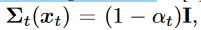
\includegraphics{E:/Learning/MyObsidian/MyObsidian/Pasted image 20231130091914.png}
  \item
    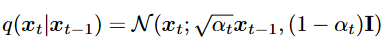
\includegraphics{E:/Learning/MyObsidian/MyObsidian/Pasted image 20231130091944.png}
  \item
    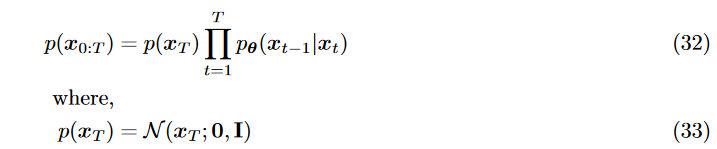
\includegraphics{E:/Learning/MyObsidian/MyObsidian/Pasted image 20231130092041.png}
  \item
    不同于HVAE, encoder过程没有参数 {} ,每一步为Gaussian. 我们关心 {}
    以生成新的{}.
  \end{enumerate}
\item
  ELBO式子

  \begin{enumerate}
  \tightlist
  \item
    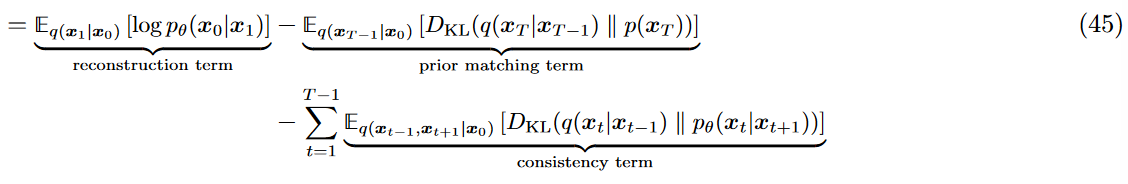
\includegraphics{E:/Learning/MyObsidian/MyObsidian/Pasted image 20231130093329.png}

    \begin{enumerate}
    \tightlist
    \item
      reconstruction:
    \item
      prior matching : 不用优化,没有learnable parameters,
      足够大T可以使最后为gaussian, 这一项变为0
    \item
      consistency term: 因此主要优化第三个式子, 然而使用Monte
      Carlo涉及两个r.v. {} ,
      会变得不稳定(这两个随机变量噪声叠加,最终估计的是加上所有采样,所以variance
      会高)
    \item
      由于{}无法求(注:推导 :{}是 given {},如果将{}看作 {}
      那么后面就是边缘概率的积分)
      利用markov化为另一种形式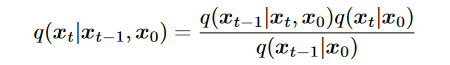
\includegraphics{E:/Learning/MyObsidian/MyObsidian/Pasted image 20231130094503.png}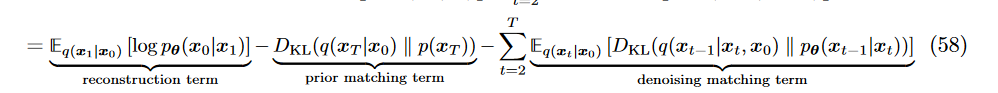
\includegraphics{E:/Learning/MyObsidian/MyObsidian/Pasted image 20231130094516.png}\\
      1. 最后一项:denosing matching. 希望denosing transition step {} 和
      ground-truth denosing transition step
      {}越接近越好。其中在HVAE由于本身encoder
      learning复杂因此{}不好计算,而在VDM中可以利用gaussian性质简化:\\
      1.
      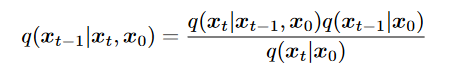
\includegraphics{E:/Learning/MyObsidian/MyObsidian/Pasted image 20231130095509.png}
      这样可以用markov, 只需要找到{}就可以。\\
      2.
      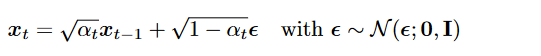
\includegraphics{E:/Learning/MyObsidian/MyObsidian/Pasted image 20231130095345.png}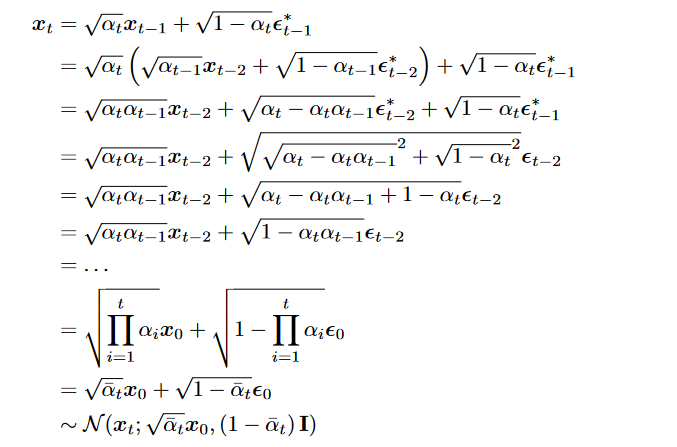
\includegraphics{E:/Learning/MyObsidian/MyObsidian/Pasted image 20231130095444.png}\\
      3.
      {}最终化为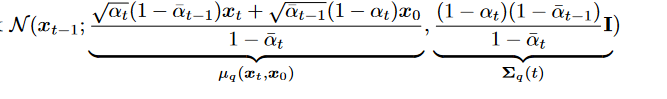
\includegraphics{E:/Learning/MyObsidian/MyObsidian/Pasted image 20231130095816.png}\\
      2. 由于 希望denosing transition step {} 和 ground-truth denosing
      transition step {}越接近越好,可以把{} 建模为Gaussian
      :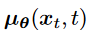
\includegraphics{E:/Learning/MyObsidian/MyObsidian/Pasted image 20231130100706.png},
      mean确定后参数确定,从而variance确定\\
      1.
      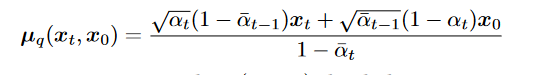
\includegraphics{E:/Learning/MyObsidian/MyObsidian/Pasted image 20231130100921.png}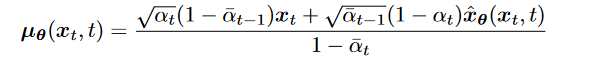
\includegraphics{E:/Learning/MyObsidian/MyObsidian/Pasted image 20231130100935.png}
      {} 由 neural network给出\\
      2.
      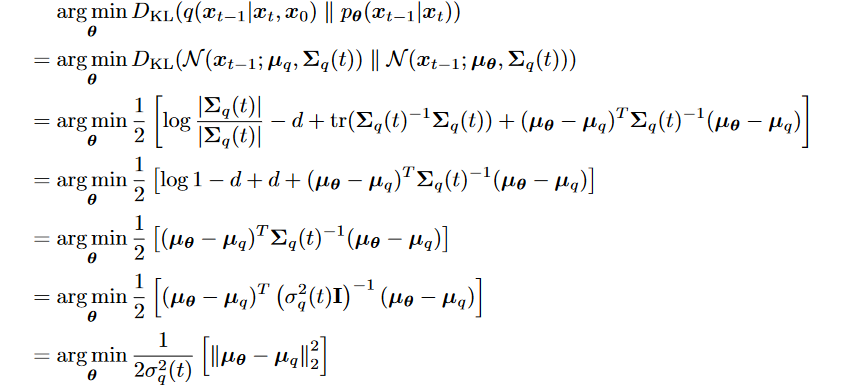
\includegraphics{E:/Learning/MyObsidian/MyObsidian/Pasted image 20231130101050.png}\\
      3.
      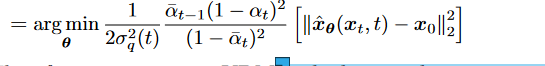
\includegraphics{E:/Learning/MyObsidian/MyObsidian/Pasted image 20231130101105.png}\\
      4. 最后是minimize expectations over all
      timesteps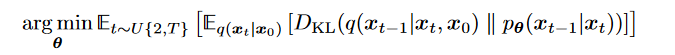
\includegraphics{E:/Learning/MyObsidian/MyObsidian/Pasted image 20231130101225.png}
    \end{enumerate}
  \end{enumerate}
\item
  Learning noise parameters

  \begin{enumerate}
  \tightlist
  \item
    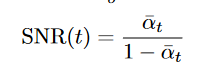
\includegraphics{E:/Learning/MyObsidian/MyObsidian/Pasted image 20231130101848.png}由前面推导得SNR,SNR越小Noise越大,希望t增加snr单调减少。
  \item
    最终可化简为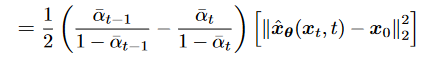
\includegraphics{E:/Learning/MyObsidian/MyObsidian/Pasted image 20231130102053.png}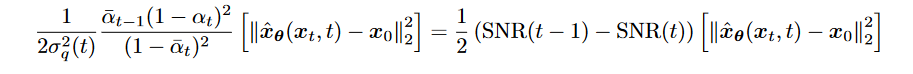
\includegraphics{E:/Learning/MyObsidian/MyObsidian/Pasted image 20231130102103.png}
  \item
    希望构建nn去model snr,
    表达为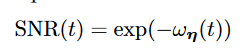
\includegraphics{E:/Learning/MyObsidian/MyObsidian/Pasted image 20231130102148.png}
  \end{enumerate}
\item
  noise形式

  \begin{enumerate}
  \tightlist
  \item
    带入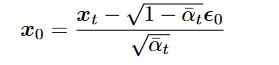
\includegraphics{E:/Learning/MyObsidian/MyObsidian/Pasted image 20231130102716.png}到
    {} ,
    得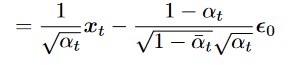
\includegraphics{E:/Learning/MyObsidian/MyObsidian/Pasted image 20231130102741.png}
  \item
    带入KL式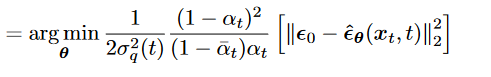
\includegraphics{E:/Learning/MyObsidian/MyObsidian/Pasted image 20231130102803.png}
  \item
    表示predict x0相当于predict noise.(一些表明predict noise
    performance更好)
  \end{enumerate}
\item
  形式

  \begin{enumerate}
  \tightlist
  \item
    Tweedie's Formula : "states that the true mean of an exponential
    family distribution, given samples drawn from it, can be estimated
    by the maximum likelihood estimate of the samples (aka empirical
    mean) plus some correction term involving the score of the
    estimate."
    矫正项考虑到sample分布情况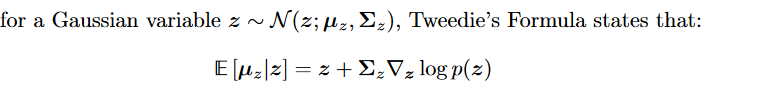
\includegraphics{E:/Learning/MyObsidian/MyObsidian/Pasted image 20231130103552.png}
  \item
    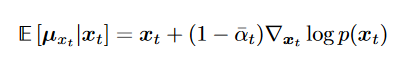
\includegraphics{E:/Learning/MyObsidian/MyObsidian/Pasted image 20231130103710.png}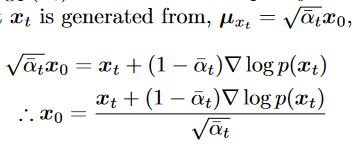
\includegraphics{E:/Learning/MyObsidian/MyObsidian/Pasted image 20231130103727.png}
  \item
    带入{} 推出:

    \begin{enumerate}
    \tightlist
    \item
      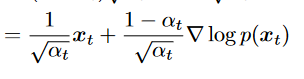
\includegraphics{E:/Learning/MyObsidian/MyObsidian/Pasted image 20231130103834.png}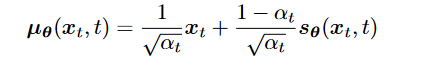
\includegraphics{E:/Learning/MyObsidian/MyObsidian/Pasted image 20231130103849.png}
    \end{enumerate}
  \item
    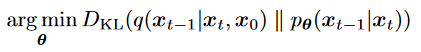
\includegraphics{E:/Learning/MyObsidian/MyObsidian/Pasted image 20231130103917.png}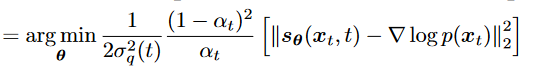
\includegraphics{E:/Learning/MyObsidian/MyObsidian/Pasted image 20231130103929.png}{}
    is a nn learns to predict the score function {}
  \item
    和原来{} 关系?:可见多一个scale项,score function
    指导我们如何在数据空间中移动以优化(最大化)目标函数(这里是log
    p)的作用,intuitively,是添加source noise 的反方向

    \begin{enumerate}
    \tightlist
    \item
      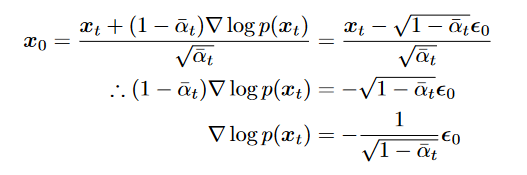
\includegraphics{E:/Learning/MyObsidian/MyObsidian/Pasted image 20231130104036.png}
    \end{enumerate}
  \end{enumerate}
\end{enumerate}

\subsubsection{DDPM}\label{ddpm}

\paragraph{扩散}\label{ux6269ux6563}

{}{}{}

\paragraph{反向}\label{ux53cdux5411}

{} {}{}

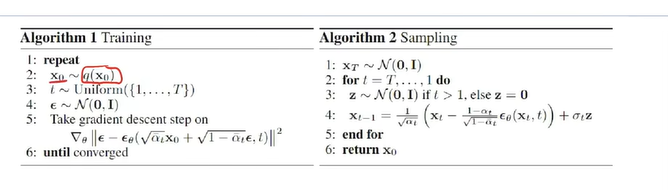
\includegraphics{E:/Learning/MyObsidian/MyObsidian/Pasted image 20240223110641.png}\\
注:

\section{ControlNet}\label{controlnet}

\subsection{Motivation}\label{motivation}

\begin{enumerate}
\tightlist
\item
  希望能用额外的图像特定构图(, edge maps, human pose skeletons,
  segmentation maps, depth, normals,)
\item
  对大型的T2I模型来讲,学习end-to-end条件的控制具有的挑战:

  \begin{enumerate}
  \tightlist
  \item
    训练学习特定的条件的训练数据较小,会导致overfitting and catastrophic
    forgetting
  \end{enumerate}
\end{enumerate}

\subsection{Contribution}\label{contribution}

\begin{enumerate}
\tightlist
\item
  锁定原来参数:
\item
  对一部分encoder layer做trainnable copy
\item
  两个部分通过zero convolution
  layer连接(防止有害的噪声干扰diffusion训练)
\end{enumerate}

\subsection{Method}\label{method}

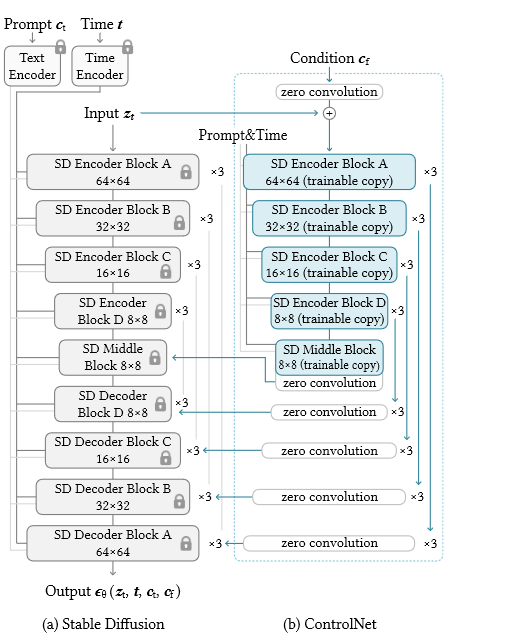
\includegraphics{E:/Learning/MyObsidian/MyObsidian/Pasted image 20240226112350.png}\\
{}:feature map {}: conditionnal vector\\
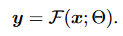
\includegraphics{E:/Learning/MyObsidian/MyObsidian/Pasted image 20240226112411.png}\\
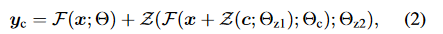
\includegraphics{E:/Learning/MyObsidian/MyObsidian/Pasted image 20240226112419.png}

\begin{enumerate}
\tightlist
\item
  初始zero conv为0,所以{},没有有害的noise可以影响隐藏层
\item
  trainable copy: 12 encoding blocks,1 moddle block
\item
  Controlnet结果通过decoder 12个skip connection加在原来网络
\item
  注意SD是将512 x 512转为 64x64作为latent
  images去训练,为了一致需要一个小的网络将条件c也embedd
\end{enumerate}

\subsection{Training}\label{training}

\begin{enumerate}
\tightlist
\item
  用empty
  string随机替换50\%text-\textgreater 增加ControlNet对conditioning
  image语义识别能力 (??CFG)
\item
  一个观察:sudden convergence phenomenon
  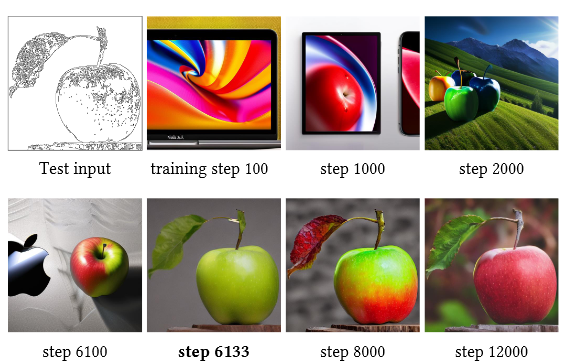
\includegraphics{E:/Learning/MyObsidian/MyObsidian/Pasted image 20240227201530.png}
\end{enumerate}

\subsection{Inference}\label{inference}

\subsubsection{CFG}\label{cfg}

\includegraphics{E:/Learning/MyObsidian/MyObsidian/Pasted image 20240228162258.png}\\
conditioning image :

\begin{enumerate}
\tightlist
\item
  加在uc和c: 当无prompt时,同时加会移除guidance
\item
  加在c: 使得guidance过强,图像过饱和\\
  解决:加在c,并且在加到SD上时根据13个block大小乘上系数,降低image
  guidance
\end{enumerate}

\subsubsection{多个controlnet}\label{ux591aux4e2acontrolnet}

每个单独训练,最后相加

\subsection{实验}\label{ux5b9eux9a8c}

\subsection{Ablative study}\label{ablative-study}

说明trainable copy和zero conv有效性 :1)trainable copy换为conv
2)zero换Gaussian\\
\includegraphics{E:/Learning/MyObsidian/MyObsidian/Pasted image 20240228164008.png}

\subsubsection{评估}\label{ux8bc4ux4f30}

\begin{itemize}
\tightlist
\item
  user study
\item
  ADE20K : to evaluate the conditioning fidelity.
\item
  FID,CLIP-score,CLIP aesthetic score: distribution distance
\end{itemize}

\includegraphics{E:/Learning/MyObsidian/MyObsidian/Pasted image 20240228164527.png}\\
\includegraphics{E:/Learning/MyObsidian/MyObsidian/Pasted image 20240228164546.png}

\section{DreamBooth}\label{dreambooth}

new concept learning(subject-driven)

\subsection{Motivation}\label{motivation-1}

\begin{itemize}
\tightlist
\item
  希望生成具有特定物体的图像:虽然T2I具有语义先验,但输出域表达有限(不能生成same
  subject,不准确).以往受限于global editing,没法fine-grained control
\end{itemize}

\subsection{Contribution}\label{contribution-1}

\begin{itemize}
\tightlist
\item
  fine-tune T2I :

  \begin{itemize}
  \tightlist
  \item
    text
    prompt带有关于特定物体的identifier,使模型学习到先验,这个先验和特定实体绑定。
  \item
    为防止lauguage shift: autogenous, class-specific prior preservation
    loss
  \end{itemize}
\end{itemize}

\subsection{Method}\label{method-1}

\includegraphics{E:/Learning/MyObsidian/MyObsidian/Pasted image 20240301204445.png}

\subsubsection{T2I}\label{t2i}

c: conditioning vector\\
\includegraphics{E:/Learning/MyObsidian/MyObsidian/Pasted image 20240228180146.png}

\subsubsection{Personalization}\label{personalization}

\begin{enumerate}
\item
  相比于GANs的fine-tune易导致overfit和mode-collapse:

  \begin{quote}
  large text-to-image diffusion models seem to excel at integrating new
  information into their domain without forgetting the prior or
  overfitting to a small set of training images.
  \end{quote}
\end{enumerate}

\subsubsection{Prompt}\label{prompt}

a {[}identifier{]} {[}class noun{]}

\subsubsection{Identifier}\label{identifier}

需要identifier在LM和diffusion中都具有weak prior.

\begin{itemize}
\tightlist
\item
  rare identifier: {}, f: tockenizer; {}: decoded text
\item
\end{itemize}

\subsubsection{Class-specific Prior Preservation
Loss}\label{class-specific-prior-preservation-loss}

\begin{itemize}
\tightlist
\item
  Fine-tune Problem:

  \begin{itemize}
  \tightlist
  \item
    finetune 可能带来lauguage drift

    \begin{itemize}
    \tightlist
    \item
      (注:LM
      finetune后失去原先的句法语义知识,diffusion也有相似现象``slowly
      forgets how to generate subjects of the same class as the target
      subject'')
    \end{itemize}
  \item
    减少了diversity
  \end{itemize}
\item
  解决上述两问题:loss

  \begin{itemize}
  \tightlist
  \item
    另外用{[}class noun{]}生成数据 {}
  \item
    \includegraphics{E:/Learning/MyObsidian/MyObsidian/Pasted image 20240228182558.png}

    \begin{itemize}
    \tightlist
    \item
      第二项prior-preservation
      term:用生成的数据来指导模型,以保持先验信息
    \end{itemize}
  \end{itemize}
\end{itemize}

\subsection{Experiments}\label{experiments}

评估:

\begin{itemize}
\tightlist
\item
  subject fidelity:

  \begin{itemize}
  \tightlist
  \item
    CLIP-I : average pairwise cosine similarity between CLIP embeddings
    of generated and real images(但不能区分高度相似文本的物体)
  \item
    DINO: 鼓励区分物体独特特征
  \end{itemize}
\item
  prompt fidelity\\
  + CLIP-T: average pairwise cosine similarity between CLIP embeddings
  of generated and real images\\
  \includegraphics{E:/Learning/MyObsidian/MyObsidian/Pasted image 20240228183541.png}\\
  在Imagen上比在SD上好
\end{itemize}

\subsubsection{消融实验}\label{ux6d88ux878dux5b9eux9a8c}

\begin{itemize}
\tightlist
\item
  Prior preservation loss
\item
  class-prior
\item
\end{itemize}

\subsubsection{局限性}\label{ux5c40ux9650ux6027}

\begin{itemize}
\tightlist
\item
  没能根据context生成正确背景

  \begin{itemize}
  \tightlist
  \item
    可能这些a weak prior for contexts,或在数据集中这些概念共现概率低
  \end{itemize}
\item
  context-appearance entanglement:物体跟随背景变化了
\item
  overfitting to the real images:prompt和training
  set中图片的setting较像
\item
  一些常见的物体更容易学习
\end{itemize}

\section{Null-text Inversion}\label{null-text-inversion}

\includegraphics{E:/Learning/MyObsidian/MyObsidian/Pasted image 20240301204752.png}\\
Inversion: 通过优化uncond 中的null-text

\end{document}
